\documentclass[16pt]{beamer}
\usepackage[utf8]{inputenc}
\usepackage{pgfpages}
\usepackage{chngpage}
\usepackage{calc}
\RequirePackage[absolute, overlay]{textpos}

\title{Bonnes pratiques à l'ère du numérique}
\setbeameroption{show notes on second screen=right}
\usetheme{default}

\usepackage[utf8]{inputenc}
\usepackage{amsmath}
\usepackage{amsfonts}
\usepackage{amssymb}
\usepackage{pgf}
\usepackage{color}
\usepackage[frenchb]{babel}
\usepackage{amssymb}
\usepackage{hyperref}

\usefonttheme{default}
\usepackage{DejaVuSans}
%\usepackage[sfdefault]{FiraSans} %% option 'sfdefault' activates Fira Sans as the default text font
\usepackage[T1]{fontenc}
\renewcommand*\oldstylenums[1]{{\firaoldstyle #1}}


\setbeamertemplate{navigation symbols}{} %remove navigation symbols

\author{Cédric Jeanneret (aka \href{https://www.twitter.com/SwissTengu}{@SwissTengu})}
\institute{\href{https://www.ethack.org/}{EthACK.org}}
\date{\today}

\definecolor{linecolor}{HTML}{4d4c4c}

\setbeamercolor{linecolor}{fg=white,bg=linecolor}

\setbeamertemplate{headline} {
	\begin{beamercolorbox}[wd=\paperwidth,dp=8pt,ht=12pt,leftskip=.29cm,rightskip=.29cm]{linecolor}
	\hfill
	\hypersetup{
		colorlinks=true,
		linkcolor=white,
		urlcolor=white,
	}
	\insertinstitute
	\end{beamercolorbox}%
}

\setbeamertemplate{footline}{%
	\begin{beamercolorbox}[wd=\paperwidth,dp=9pt,ht=0.4cm,leftskip=.29cm,rightskip=.3cm]{linecolor}
	\pgfputat{\pgfxy(0.455,-0.315)}{\pgfbox[center,base]{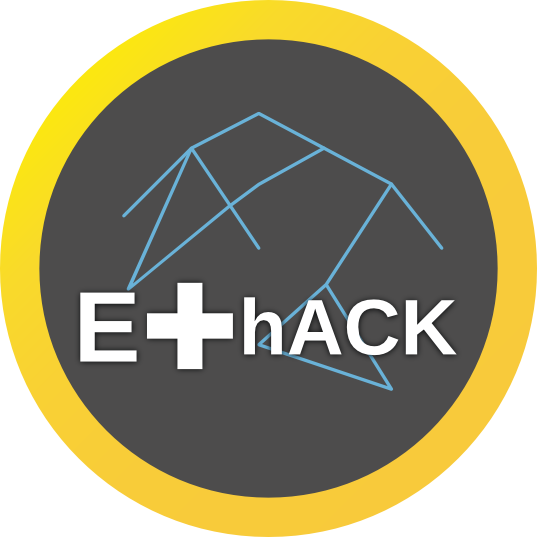
\includegraphics[width=1.5cm]{../common/logo_537.png}}}
	\hfill
	\inserttitle
	\end{beamercolorbox}%
}


\hypersetup{
	colorlinks=true,
	linkcolor=blue,
	urlcolor=blue,
	pdfborderstyle={/S/U/W 1},
	pdfborder=0 0 1,
	linkbordercolor={0 0 0},
	urlbordercolor={0 0 0},
}


\begin{document}

{
\setbeamertemplate{footline}{%
	\begin{beamercolorbox}[wd=\paperwidth,dp=8pt,ht=12pt,leftskip=.29cm,rightskip=.3cm]{linecolor}
	\hfill
	\inserttitle
	\end{beamercolorbox}%
}

% center first slide — not a title, but almost
{
\centering
\begin{frame}

EthACK
\vspace{0.5cm}

The Swiss Privacy Basecamp 
\vspace{0.5cm}

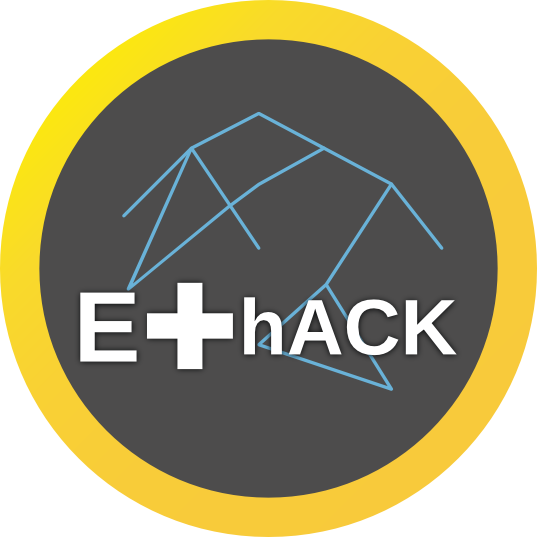
\includegraphics[width=4cm]{../common/logo_537.png}

\end{frame}
}
}

\begin{frame}{EthACK ?}
\begin{itemize}
	\item Éthique
	\item État
	\item ACKnowledgement (reconnaissance)
	\item Hacking (éthique, évidemment)
	\item …
\end{itemize}
\end{frame}

\begin{frame}{Pourquoi ?}
\begin{itemize}
	\item Notre gouvernement ne s'intéresse pas (ou peu) au sujet
	\item Les sociétés privées nous fichent à notre insu
	\item Personne ne sait où sont leurs données, qui les traitent, à quoi elles servent
\end{itemize}
\end{frame}


\begin{frame}
  \titlepage
\end{frame}

\begin{frame}
{Plan}
\begin{itemize}
\item Les utilisations et menaces
\item (Pause / Questions)
\item De l'hygiène numérique
\item (Questions et fin)
\end{itemize}
\end{frame}

\begin{frame}
{Numérique présent partout}
\begin{itemize}
\item Smartphone
\item Ordinateur portable
\item Smartwatch
\item Électroménager
\item jouets
\item …
\end{itemize}
\note<1>[item]{On ne peut plus s'en passer}
\note<1>[item]{Arrive partout, maison, voiture, loisirs, etc}
\note<1>[item]{Sommes-nous prêt-e-s ?}
\end{frame}

\begin{frame}
{Utilisations}
\begin{itemize}
\item Communication (pro/privé)
\item Apprentissage / extension des connaissances
\item Organisation
\item Loisirs
\item …
\end{itemize}
\note<1>[item]{Sécurité (caméras de surveillance, etc)}
\note<1>[item]{anecdote IoT employé dans le cadre du DDoS OVH (145'000 caméras)}
\note<1>[item]{On va se concentrer sur "communication" - source de problèmes divers et variés}
\end{frame}

\begin{frame}
{}
\center
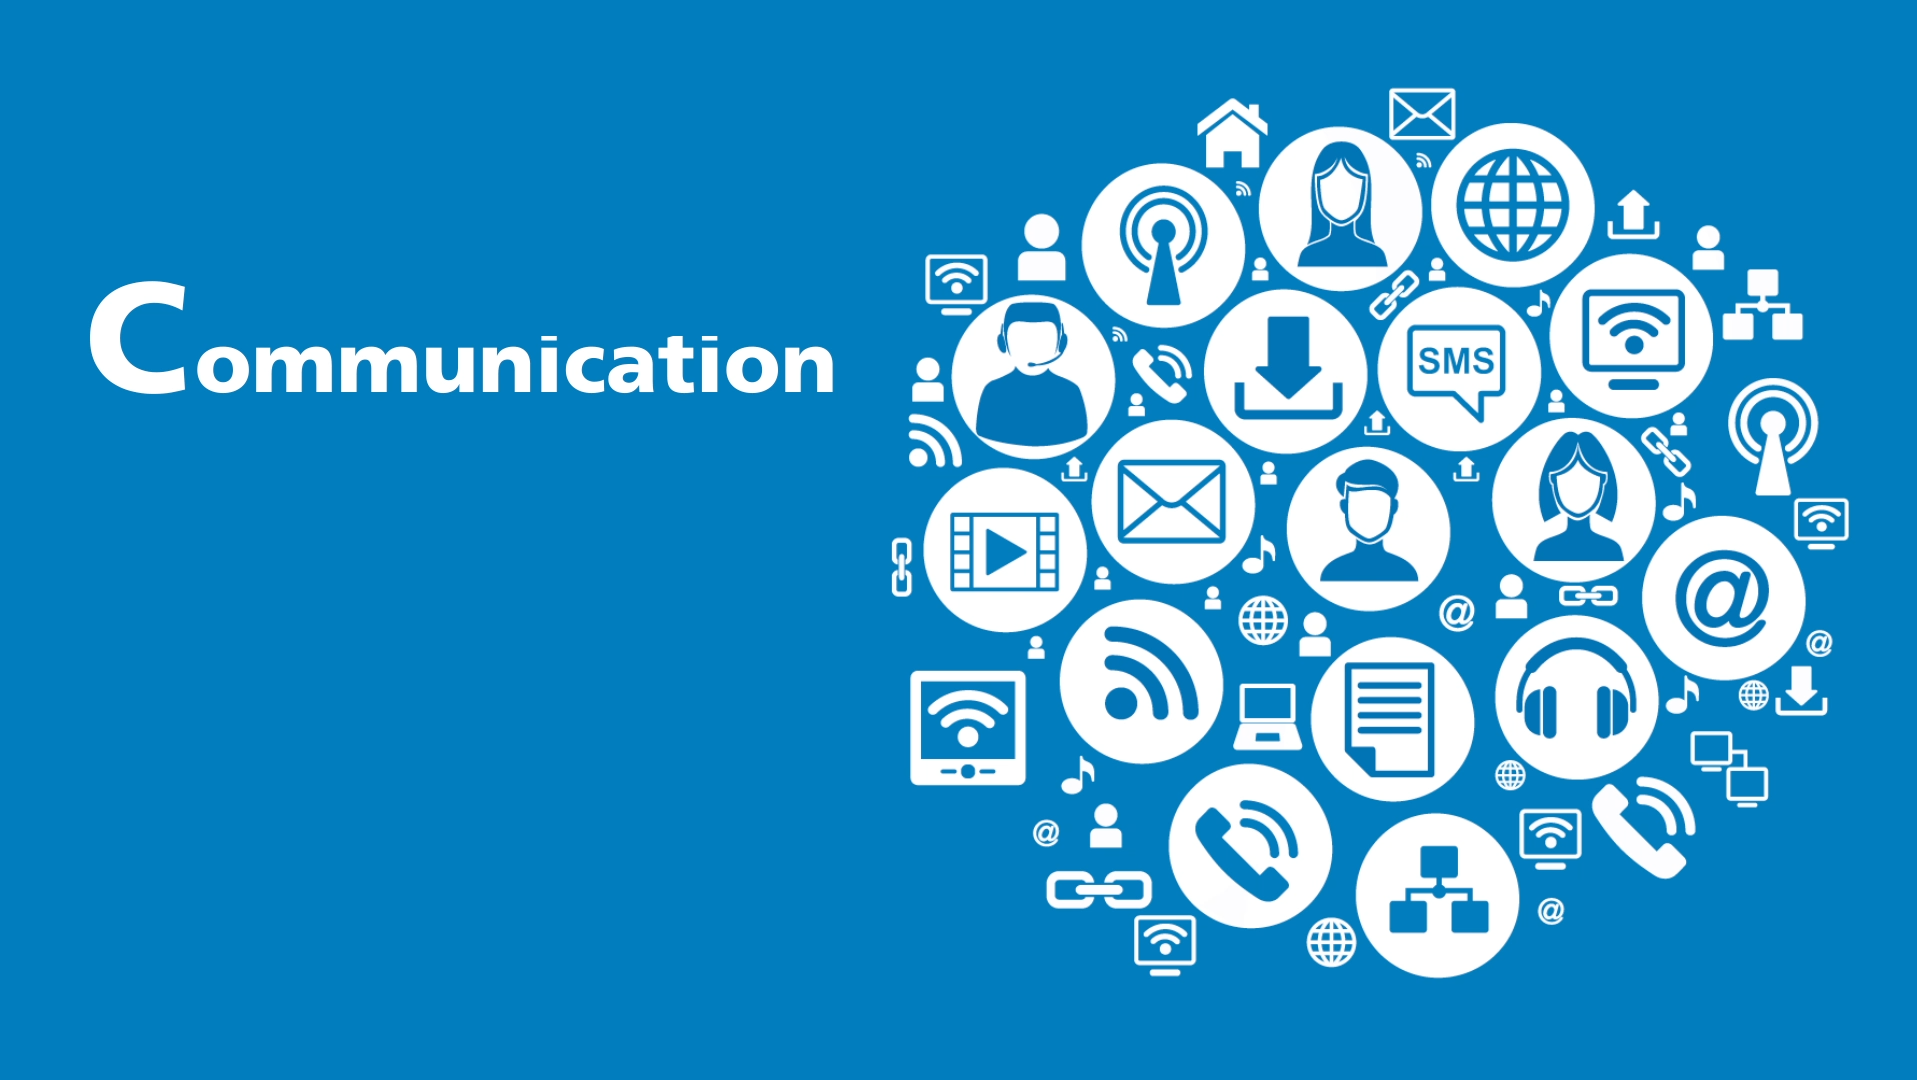
\includegraphics[width=\textwidth, height=\textheight,keepaspectratio]{communication.png}
\note<1>{Pourquoi la communication ? quantité de moyens, les interactions profs/élèves, élèves/élèves, parents. Responsabilités dans le cadre scolaire, etc}
\end{frame}

\begin{frame}
{Communication}
\begin{itemize}
\item SMS
\note<1>[item]{Plus tant employé, mais encore présent pour de l'authentification (e-banking par exemple)}
\item Messageries instantanées
\begin{itemize}
\item Whatsapp
\item Facebook Messenger
\item Telegram
\item Threema
\item …
\end{itemize}
\note<1>[item]{Le truc actuel, passe par Internet, simple et efficace}
\item E-Mails
\note<1>[item]{Non, il n'y a pas que le spam…}
\end{itemize}
\end{frame}

\begin{frame}
{}
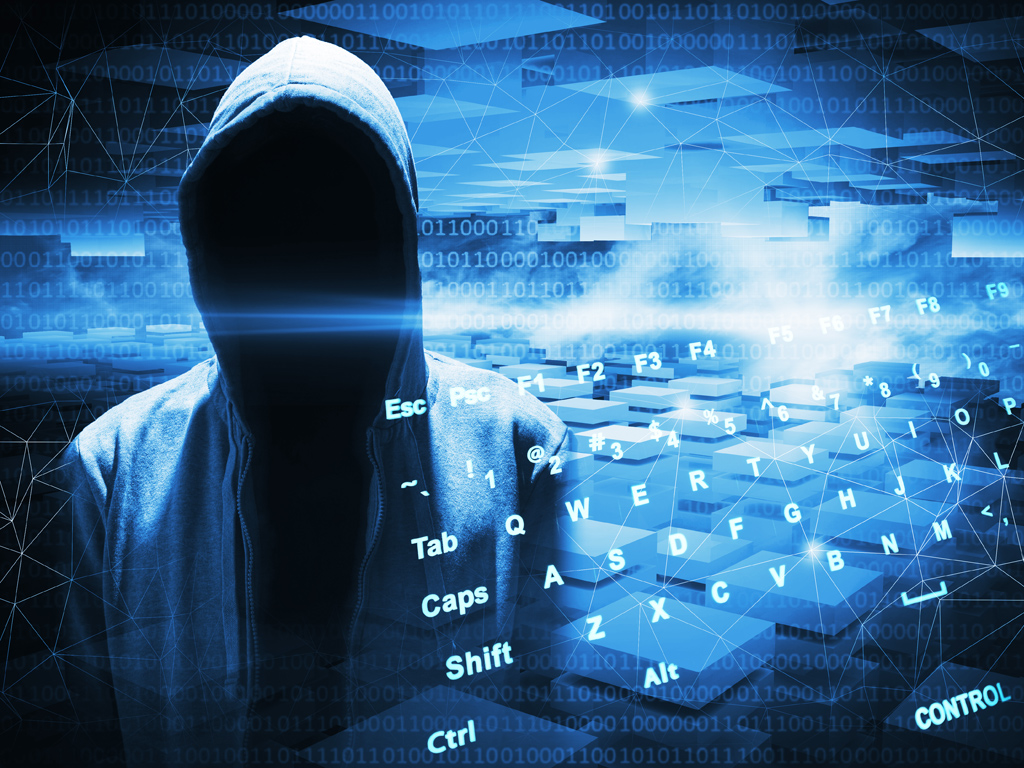
\includegraphics[width=\textwidth,height=\textheight,keepaspectratio]{hacker-05-shutterstock.jpg}
\note<1>[item]{Menaces diverses et variées sur chacun de ces moyens}
\end{frame}

\begin{frame}
{Menaces sur la communication}
\begin{itemize}
\item Interception/modification des contenus
\item Usurpation d'identité
\item Perte/vol de l'appareil
\item Vol des codes d'accès
\item …
\note<1>[item]{Dans le cadre scolaire : usurpation + vol sont des gros risques}
\note<1>[item]{Attention aux accès wifi "gratuits", "ouverts", etc.}
\note<1>[item]{Rappeler les proxy filtrants sur le réseau scolaire, avec la CA swisscom…}
\end{itemize}
\end{frame}

\begin{frame}
{Le plus courant (pour le moment)}
\begin{itemize}
\item Perte/vol (de l'appareil)
\item Phishing (vol des identifiants/information)
\item "Oublier" ouvert sur une table
\item "Partage" de session
\end{itemize}
\note<1>{Rappeler qu'aucun service digne de ce nom ne demande jamais les identifiants par mail…}
\note<1>{Rappeler qu'un élève peut être assez dégourdi pour regarder le contenu}
\note<1>{Noter en passant que l'interception légale va devenir monnaie courante (LRens)}
\end{frame}

\begin{frame}
{L'appareil n'y peut rien}
\center{
L'appareil (ordinateur, smartphone, etc) fait strictement ce qu'on lui dit de faire}

\note<1>[item]{L'utilisateur est seul responsable de l'usage qu'il en fait}
\note<1>[item]{L'utilisateur doit protéger ses appareils}
\note<1>[item]{Interaction : combien ont un PIN sur leur smartphone}
\end{frame}

\begin{frame}
{}
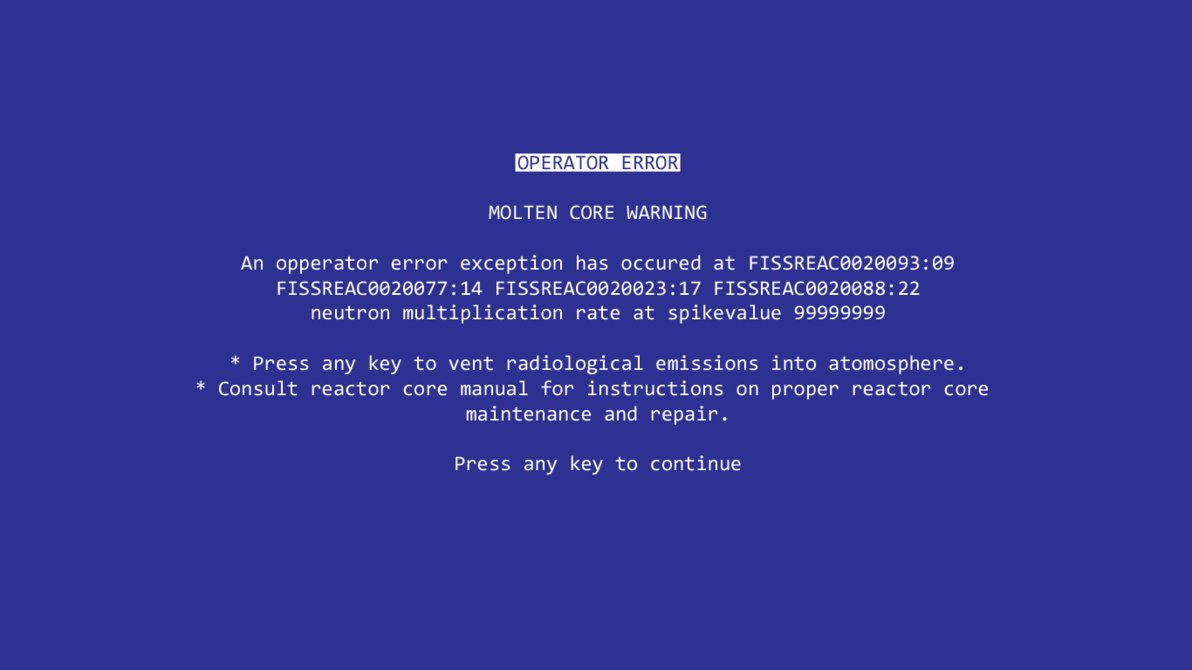
\includegraphics[width=\paperwidth,height=\paperheight]{bsod.png}
\note<1>{Des fois, ça décide de planter, aussi}
\end{frame}

\begin{frame}
{Appareil privé…}

\begin{itemize}
\item Vos contacts
\item Vos jeux
\item Vos comptes
\end{itemize}
\end{frame}

\begin{frame}
{… mais aussi employé au boulot}
\begin{itemize}
\item Les contacts professionnels
\item Accès aux jeux/autres dans le milieu professionnel
\item Vos comptes privés mélangés à ceux du travail
\end{itemize}
\end{frame}

\begin{frame}
{Tout va bien :)}
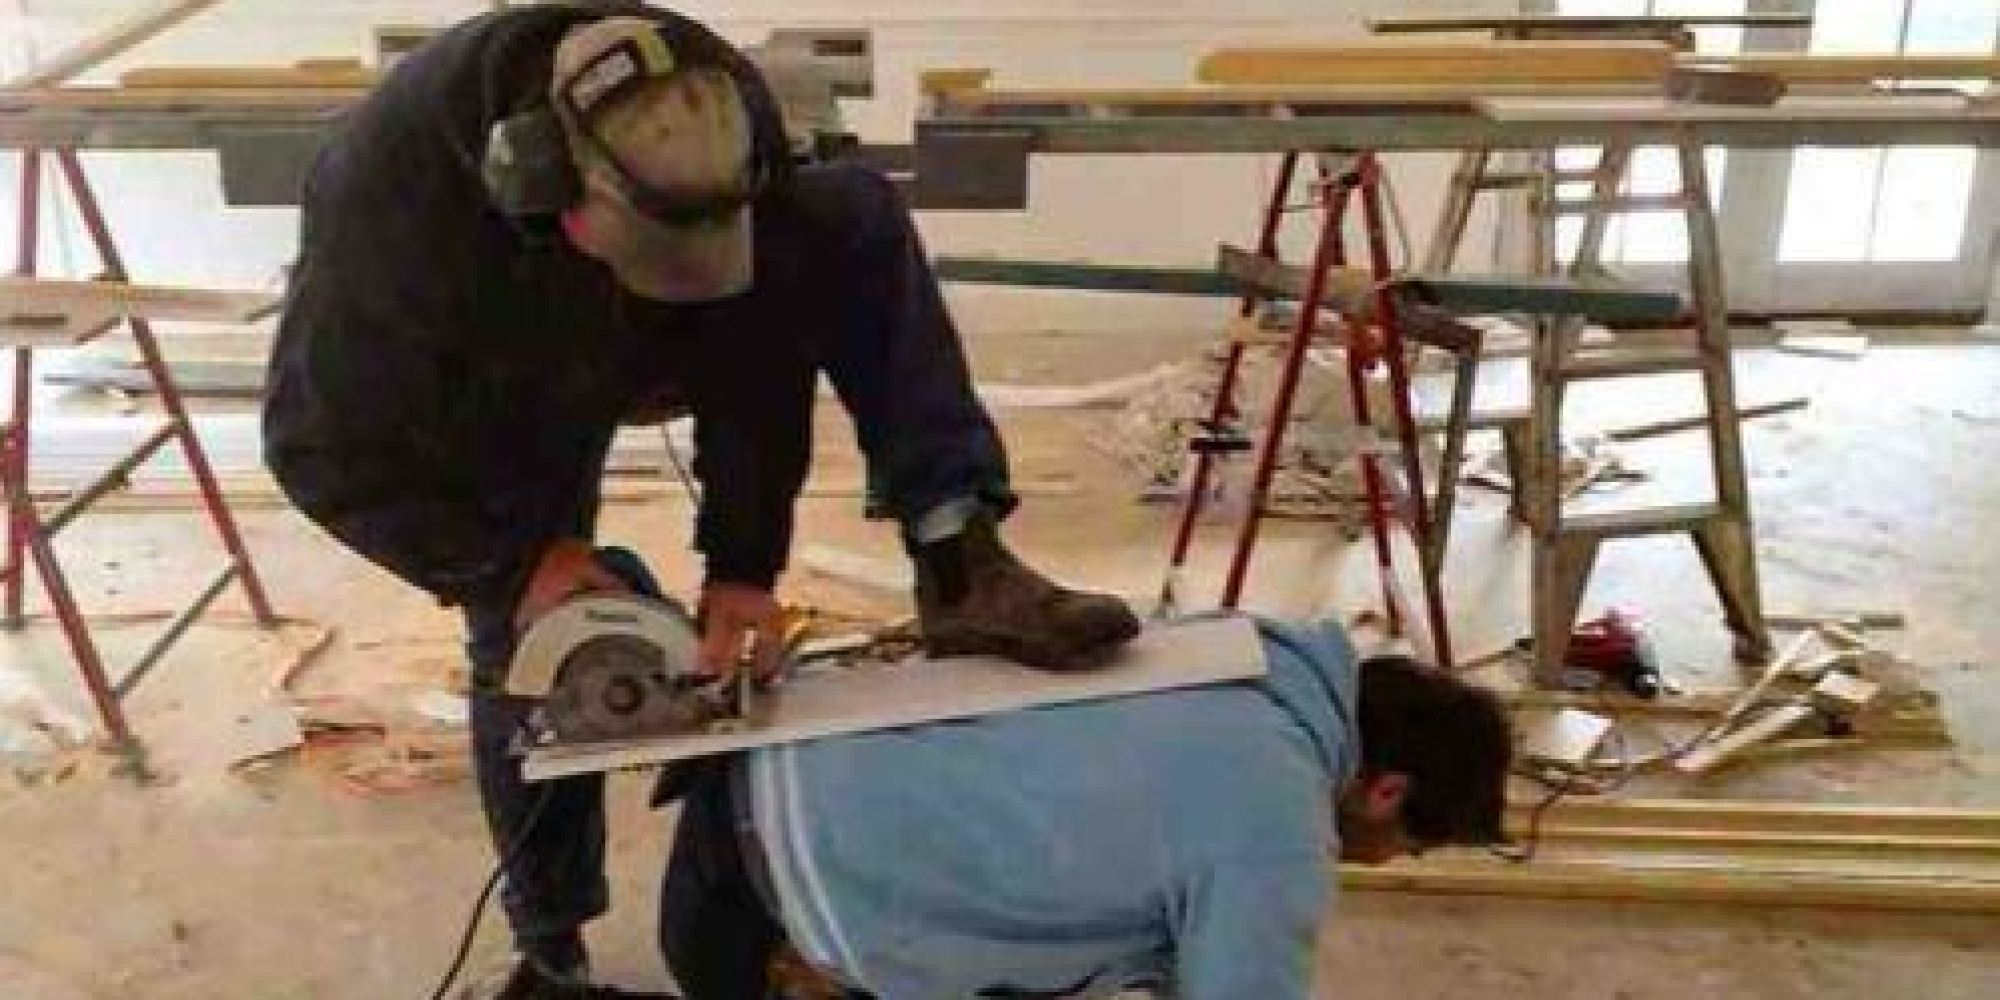
\includegraphics[width=\textwidth,height=\textheight,keepaspectratio]{what-could-go-wrong.jpg}
\end{frame}

\begin{frame}
{Oui, après tout, qu'est-ce qui peut se passer ?}
\begin{itemize}
\item Perte/vol de l'appareil
\item Appareils fragiles : cassés
\item …, etc
\end{itemize}
Le tout avec des données professionnelles, des accès, des informations, etc

\note<1>{Sans parler de la séparation pro/privée — exemple du verre de minuit}
\end{frame}

\begin{frame}
{}
\center
Et les Réseaux Sociaux ?
\note<1>[item]{Transfert de données personnelles (bidirectionnel)}
\note<1>[item]{Quid de la neutralité/impartialité ?}
\note<1>[item]{Possible "concours" entre élèves (cf Periscope)}
\note<1>[item]{Implication plus personnelle/émotionnelle possible}
\note<1>[item]{Interactif: combien sont "amis" avec leurs élèves sur Facebook}
\end{frame}

\begin{frame}
{Questions, pause clope, etc}
\end{frame}

\begin{frame}
{Hygiène numérique}
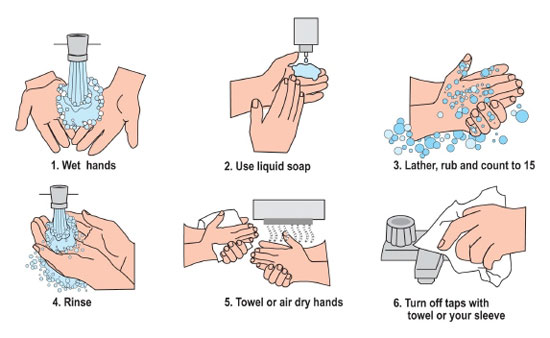
\includegraphics[width=\textwidth,height=\textheight,keepaspectratio]{how-to-wash-your-hands.jpg}
\note<1>{La vie numérique, c'est comme la vraie vie, faut se laver, s'assurer qu'on a un aspect soigné.}
\end{frame}

\begin{frame}
{Quelques notions élémentaires}
\begin{itemize}
\item Les actions "physiques" impactent le "monde numérique"
\item Les actions "numériques" impactent le "monde physique"
\item Garder en tête la notion de "Citoyen Numérique"
\end{itemize}
\end{frame}
\begin{frame}
{}
\center
Tourner sept fois le clavier dans la bouche avant d'envoyer
\end{frame}

\begin{frame}
{Ton smartphone tu sécuriseras}
  \begin{columns}[T]
    \begin{column}{.25\textwidth}
     \begin{block}{}
	   
\includegraphics[width=2cm,keepaspectratio]{Yoda-Wisdom.jpg}
     \end{block}
    \end{column}
    \begin{column}{.75\textwidth}
    \begin{block}{}
		\begin{itemize}
		\item Code pin
		\item Services annexes
		\item Bluetooth
		\item NFC
		\item Surveillance
		\end{itemize}
    \end{block}
    \end{column}
  \end{columns}

\note<1>[item]{Un code pin pour l'allumer, et débloquer l'écran}
\note<1>[item]{Est-ce que les 10'000 trucs à côté sont réellement nécessaires ? Il y a-t-il des mots de passe corrects ?}
\note<1>[item]{Bluetooth = porte dérobée permettant de faire pas mal de choses}
\note<1>[item]{NFC : pareil que BT}
\note<1>[item]{Un smartphone ne se laisse pas sans surveillance - la poche/sac = meilleur ami ! (poche arrière: danger :])}
\end{frame}

\begin{frame}
{Les services tu trieras}
  \begin{columns}[T]
    \begin{column}{.25\textwidth}
     \begin{block}{}
	   
\includegraphics[width=2cm,keepaspectratio]{Yoda-Wisdom.jpg}
     \end{block}
    \end{column}
    \begin{column}{.75\textwidth}
    \begin{block}{}
		\begin{itemize}
		\item Cloud
		\item Messageries instantanées
		\item Jeux et autres apps
		\item Norme PEGI
		\end{itemize}
    \end{block}
    \end{column}
  \end{columns}

\note<1>[item]{Services de synchro : utiles ? Sécurisés (mdp) ? De confiance ?}
\note<1>[item]{Telegram, WhatsApp, etc : réellement utiles ? Utilisation correcte ? Séparation claire pro/privé ?}
\note<1>[item]{Droits des apps sur vos données ? Accès de ces apps au réseau ? Partage potentiels avec des élèves (localisation) ?}
\note<1>[item]{PEGI => norme à l'échelle UE - chiffre == âge minimal pour le contenu, jeu/vidéo}
\end{frame}

\begin{frame}
{Tes appareils privés tu ne prêteras pas}
  \begin{columns}[T]
    \begin{column}{.25\textwidth}
     \begin{block}{}
	   
\includegraphics[width=2cm,keepaspectratio]{Yoda-Wisdom.jpg}
     \end{block}
    \end{column}
    \begin{column}{.75\textwidth}
    \begin{block}{}
		\begin{itemize}
		\item Pas sans surveillance
		\item Sur une session utilisateur dédiée
		\item Est-ce vraiment nécessaire "maintenant tout de suite ?"
		\end{itemize}
    \end{block}
    \end{column}
  \end{columns}

\note<1>[item]{S'assurer que "l'invité" fasse ce qu'il a dit}
\note<1>[item]{S'assurer que les droits d'accès évitent les problèmes (mail, fichiers, etc)}
\note<1>[item]{Après tout, ça peut sans doute attendre le soir chez soi non ?}
\note<1>[item]{En aucun cas un smartphone/tablette ne devrait être prêté - trop de risques pour les données dessus}
\end{frame}

\begin{frame}
{Un mot de passe solide tu choisira}
  \begin{columns}[T]
    \begin{column}{.25\textwidth}
     \begin{block}{}
	   
\includegraphics[width=2cm,keepaspectratio]{Yoda-Wisdom.jpg}
     \end{block}
    \end{column}
    \begin{column}{.75\textwidth}
    \begin{block}{}
		\begin{itemize}
		\item "Phrase de passe"
		\item Pas une date/lieu de référence
		\item Le nom du chien n'est pas une bonne idée
		\item Pas de réutilisation de mot de passe !
		\end{itemize}
    \end{block}
    \end{column}
  \end{columns}
  \note<1>[item]{Une phrase est mieux qu'une suite de caractère (mémoire)}
  \note<1>[item]{Les dates/lieux sont trouvables (RS)}
  \note<1>[item]{Les noms sont trouvables (RS)}
  \note<1>[item]{Employer le même mot de passe partout : bad, bad, bad (hacks des services)}
\end{frame}

\begin{frame}
{}

\includegraphics[width=\textwidth,height=\textheight,keepaspectratio]{size-does-matter.jpg}
\end{frame}

\begin{frame}
{Professeurs et parents : en première ligne face aux jeunes}
\begin{itemize}
\item Montrer l'exemple
\item Se renseigner, s'informer
\item Se maintenir à jour et communiquer avec les collègues et les parents
\end{itemize}
\note<1>[item]{Oui, une tâche de plus dans le planning surchargé… désolé}
\note<1>[item]{Être exigeant avec soi-même et les autres}
\note<1>[item]{Ce "monde" avance très vite}
\note<1>[item]{Interactif: Pokemon Go : que faire, comment agir ?}
\end{frame}


{
\setbeamertemplate{footline}{%
	\begin{beamercolorbox}[wd=\paperwidth,dp=8pt,ht=12pt,leftskip=.29cm,rightskip=.3cm]{linecolor}
	\hfill
	\inserttitle
	\end{beamercolorbox}%
}
{
\centering
\begin{frame}
{Questions ?}

\href{https://ethack.org/}{https://ethack.org/} \\
\vspace{0.3cm}
\href{https://www.twitter.com/EthACK_org}{@EthACK\_org} on Twitter \\
\vspace{0.3cm}
\href{https://www.facebook.com/ethack.org}{ethack.org} on Facebook

\vspace{0.5cm}

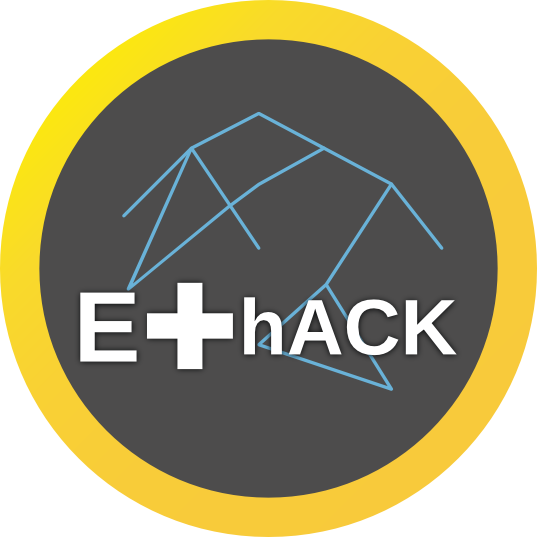
\includegraphics[width=4cm]{../common/logo_537.png}
\end{frame}
}
}

\end{document}
